% Options for packages loaded elsewhere
\PassOptionsToPackage{unicode}{hyperref}
\PassOptionsToPackage{hyphens}{url}
%
\documentclass[
  ignorenonframetext,
]{beamer}
\usepackage{pgfpages}
\setbeamertemplate{caption}[numbered]
\setbeamertemplate{caption label separator}{: }
\setbeamercolor{caption name}{fg=normal text.fg}
\beamertemplatenavigationsymbolsempty
% Prevent slide breaks in the middle of a paragraph
\widowpenalties 1 10000
\raggedbottom
\setbeamertemplate{part page}{
  \centering
  \begin{beamercolorbox}[sep=16pt,center]{part title}
    \usebeamerfont{part title}\insertpart\par
  \end{beamercolorbox}
}
\setbeamertemplate{section page}{
  \centering
  \begin{beamercolorbox}[sep=12pt,center]{part title}
    \usebeamerfont{section title}\insertsection\par
  \end{beamercolorbox}
}
\setbeamertemplate{subsection page}{
  \centering
  \begin{beamercolorbox}[sep=8pt,center]{part title}
    \usebeamerfont{subsection title}\insertsubsection\par
  \end{beamercolorbox}
}
\AtBeginPart{
  \frame{\partpage}
}
\AtBeginSection{
  \ifbibliography
  \else
    \frame{\sectionpage}
  \fi
}
\AtBeginSubsection{
  \frame{\subsectionpage}
}
\usepackage{amsmath,amssymb}
\usepackage{lmodern}
\usepackage{iftex}
\ifPDFTeX
  \usepackage[T1]{fontenc}
  \usepackage[utf8]{inputenc}
  \usepackage{textcomp} % provide euro and other symbols
\else % if luatex or xetex
  \usepackage{unicode-math}
  \defaultfontfeatures{Scale=MatchLowercase}
  \defaultfontfeatures[\rmfamily]{Ligatures=TeX,Scale=1}
\fi
% Use upquote if available, for straight quotes in verbatim environments
\IfFileExists{upquote.sty}{\usepackage{upquote}}{}
\IfFileExists{microtype.sty}{% use microtype if available
  \usepackage[]{microtype}
  \UseMicrotypeSet[protrusion]{basicmath} % disable protrusion for tt fonts
}{}
\makeatletter
\@ifundefined{KOMAClassName}{% if non-KOMA class
  \IfFileExists{parskip.sty}{%
    \usepackage{parskip}
  }{% else
    \setlength{\parindent}{0pt}
    \setlength{\parskip}{6pt plus 2pt minus 1pt}}
}{% if KOMA class
  \KOMAoptions{parskip=half}}
\makeatother
\usepackage{xcolor}
\IfFileExists{xurl.sty}{\usepackage{xurl}}{} % add URL line breaks if available
\IfFileExists{bookmark.sty}{\usepackage{bookmark}}{\usepackage{hyperref}}
\hypersetup{
  pdftitle={WASH Benefits Bangladesh Analysis of Stress Biomarkers and Growth Outcomes},
  pdfauthor={Andrew Mertens},
  hidelinks,
  pdfcreator={LaTeX via pandoc}}
\urlstyle{same} % disable monospaced font for URLs
\newif\ifbibliography
\usepackage{longtable,booktabs,array}
\usepackage{calc} % for calculating minipage widths
\usepackage{caption}
% Make caption package work with longtable
\makeatletter
\def\fnum@table{\tablename~\thetable}
\makeatother
\usepackage{graphicx}
\makeatletter
\def\maxwidth{\ifdim\Gin@nat@width>\linewidth\linewidth\else\Gin@nat@width\fi}
\def\maxheight{\ifdim\Gin@nat@height>\textheight\textheight\else\Gin@nat@height\fi}
\makeatother
% Scale images if necessary, so that they will not overflow the page
% margins by default, and it is still possible to overwrite the defaults
% using explicit options in \includegraphics[width, height, ...]{}
\setkeys{Gin}{width=\maxwidth,height=\maxheight,keepaspectratio}
% Set default figure placement to htbp
\makeatletter
\def\fps@figure{htbp}
\makeatother
\setlength{\emergencystretch}{3em} % prevent overfull lines
\providecommand{\tightlist}{%
  \setlength{\itemsep}{0pt}\setlength{\parskip}{0pt}}
\setcounter{secnumdepth}{-\maxdimen} % remove section numbering
\ifLuaTeX
  \usepackage{selnolig}  % disable illegal ligatures
\fi

\title{WASH Benefits Bangladesh Analysis of Stress Biomarkers and Growth
Outcomes}
\author{Andrew Mertens}
\date{12/7/2021}

\begin{document}
\frame{\titlepage}

\begin{frame}{Motivation}
\protect\hypertarget{motivation}{}
\begin{itemize}[<+->]
\tightlist
\item
  Children who experience growth failure may never reach their maximum
  possible cognitive development and growth failure is associated with
  increased risk of mortality or long-term morbidity.
\item
  Globally, 151 million children under 5 years of age are stunted (low
  height for age).
\item
  Prenatal development and the first 2 years of life represent a
  particularly critical window for linear and ponderal growth.
\end{itemize}
\end{frame}

\begin{frame}{Background}
\protect\hypertarget{background}{}
\begin{itemize}[<+->]
\tightlist
\item
  Chronic biological stress can impair development during critical
  windows of growth.

  \begin{itemize}[<+->]
  \tightlist
  \item
    Stressful stimuli are associated with the set point, reactivity, and
    regulation of the two primary neuroendocrine axes, the sympathetic
    adrenomedullary (SAM) and the hypothalamic-pituitary- adrenal (HPA)
    axes.
  \item
    Activation of the SAM leads to increased blood pressure and heart
    rate as well as production of salivary amylase (sAA).
  \item
    The HPA axis modulates the sympathetic nervous system through the
    production of glucocorticoids, catecholamines, and cytokines.
  \item
    The production of cytokines activates the HPA axis, which responds
    by producing glucocorticoids that inhibit the HPA axis and immune
    activity.
  \end{itemize}
\end{itemize}
\end{frame}

\begin{frame}{Background}
\protect\hypertarget{background-1}{}
\begin{itemize}[<+->]
\tightlist
\item
  Cortisol is a glucocorticoid that is particularly important to the
  stress response and follows a diurnal, circadian rhythm.

  \begin{itemize}[<+->]
  \tightlist
  \item
    In children, chronic stress is associated with disruption of diurnal
    rhythm of cortisol production.
  \end{itemize}
\item
  Cortisol binds to glucocorticoid receptors that are encoded by the
  NR3C1 gene.
\item
  The NR3C1 gene is associated with early life stress, and methylation
  of this gene is associated with stress reactivity. Furthermore, excess
  levels of glucocorticoids can lead to neurological and genetic damage
  through an imbalance in the production and elimination of reactive
  oxygen species (ROS), a process known as oxidative stress.
\item
  F2-isoprostanes are a group of prostaglandin-like compounds that have
  been validated as a measure of oxidative stress.
\end{itemize}
\end{frame}

\begin{frame}{Background}
\protect\hypertarget{background-2}{}
\begin{itemize}[<+->]
\tightlist
\item
  The term ``allostatic load'' refers to the cumulative burden of
  biological stressors that are operationalized by the biomarkers
  described above in the HPA and SAM axes.
\item
  Studies investigating the relationship between allostatic load in
  children have found chronic stress to contribute to impaired growth.
\item
  Allostatic load is related with nutritional outcomes, as higher
  allostatic load is associated with increased consumption of fat and
  decreased micronutrient intake.
\item
  Furthermore, prolonged HPA-axis activity can lead to the
  overproduction of insulin and the underproduction of growth and sex
  hormones, which can alter metabolism and growth.
\item
  Chronically high glucocorticoid levels inhibit child growth through a
  decrease in bone formation, a loss in bone mineral density, and
  altered growth-plate function.
\end{itemize}
\end{frame}

\begin{frame}{Stress Measures}
\protect\hypertarget{stress-measures}{}
\begin{itemize}[<+->]
\tightlist
\item
  Urinary F2-isoprostanes (Year 1)
\item
  Salivary alpha-amylase (Year 2)
\item
  Salivary cortisol (Year 2)
\item
  Blood pressure (Year 2)
\item
  Heart rate (Year 2)
\item
  NR3C1 methylation status (Year 2)
\end{itemize}
\end{frame}

\begin{frame}{Outcomes}
\protect\hypertarget{outcomes}{}
Exact outcomes depend on timing and type of stress measurement

\begin{itemize}[<+->]
\tightlist
\item
  Primary Outcome: Concurrent or subsequent child LAZ or linear growth
  velocity
\item
  Secondary Outcome: Concurrent or subsequent child WAZ, HCZ, weight
  change, or head circumference change
\item
  Tertiary Outcomes: Concurrent or subsequent child WLZ
\end{itemize}
\end{frame}

\begin{frame}{Hypotheses}
\protect\hypertarget{hypotheses}{}
\begin{itemize}[<+->]
\tightlist
\item
  H1. Urinary F2-isoprostane measures are negatively associated with
  child growth.
\item
  H2. Salivary cortisol reactivity is positively associated with
  concurrent child growth, and sAA reactivity is negatively associated
  with concurrent child growth. Pre- and post- stressor cortisol
  concentrations are positively associated with concurrent child growth.
  Pre- and post-stressor sAA concentrations are negatively associated
  with concurrent child growth.
\item
  H3. SAM biomarker measures are negatively associated with concurrent
  child growth
\item
  H4. Glucocorticoid receptor methylation is negatively associated with
  concurrent child growth
\end{itemize}
\end{frame}

\begin{frame}{Primary findings: H1}
\protect\hypertarget{primary-findings-h1}{}
Evidence for hypothesis 1 but not the other hypotheses.

\begin{longtable}[]{@{}
  >{\raggedright\arraybackslash}p{(\columnwidth - 6\tabcolsep) * \real{0.53}}
  >{\raggedright\arraybackslash}p{(\columnwidth - 6\tabcolsep) * \real{0.13}}
  >{\raggedright\arraybackslash}p{(\columnwidth - 6\tabcolsep) * \real{0.25}}
  >{\raggedright\arraybackslash}p{(\columnwidth - 6\tabcolsep) * \real{0.09}}@{}}
\toprule
\begin{minipage}[b]{\linewidth}\raggedright
name
\end{minipage} & \begin{minipage}[b]{\linewidth}\raggedright
Outcome
\end{minipage} & \begin{minipage}[b]{\linewidth}\raggedright
Coefficient (95\% CI)
\end{minipage} & \begin{minipage}[b]{\linewidth}\raggedright
P-value
\end{minipage} \\
\midrule
\endhead
IPF(2a)-III & LAZ Year 1 & -0.11 (-0.19, -0.04) & 0* \\
& WAZ Year 1 & -0.16 (-0.26, -0.06) & 0* \\
& WLZ Year 1 & -0.14 (-0.25, -0.03) & 0.01* \\
2,3-dinor-iPF(2a)-III & LAZ Year 1 & -0.2 (-0.31, -0.1) & 0* \\
iPF(2a)-VI & LAZ Year 1 & -0.21 (-0.33, -0.09) & 0* \\
& WAZ Year 1 & -0.13 (-0.21, -0.05) & 0* \\
& WLZ Year 1 & -0.08 (-0.16, 0) & 0.05* \\
Combined urinary oxidative stress biomarkers & LAZ Year 1 & -0.32
(-0.52, -0.11) & 0* \\
& WAZ Year 1 & -0.18 (-0.27, -0.09) & 0* \\
& WLZ Year 1 & -0.11 (-0.2, -0.03) & 0.01* \\
\bottomrule
\end{longtable}
\end{frame}

\begin{frame}{Primary findings - HAZ}
\protect\hypertarget{primary-findings---haz}{}
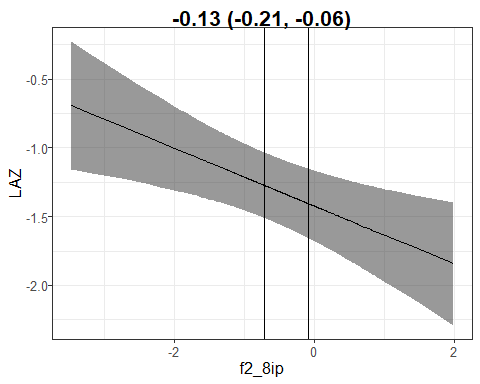
\includegraphics{stress-growth-lab-presentation_files/figure-beamer/unnamed-chunk-2-1.pdf}
\end{frame}

\begin{frame}{Exposure-response: Concurrent f2 8ip and LAZ}
\protect\hypertarget{exposure-response-concurrent-f2-8ip-and-laz}{}
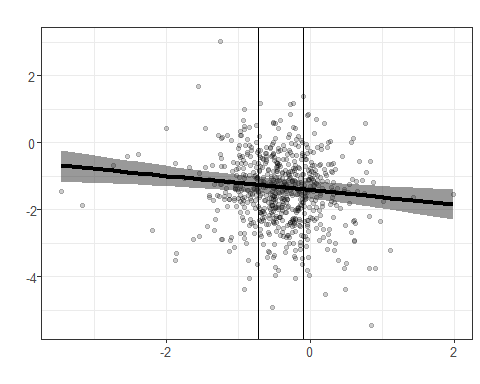
\includegraphics{stress-growth-lab-presentation_files/figure-beamer/unnamed-chunk-3-1.pdf}
\end{frame}

\begin{frame}{Exposure-response: Concurrent f2 8ip and LAZ}
\protect\hypertarget{exposure-response-concurrent-f2-8ip-and-laz-1}{}
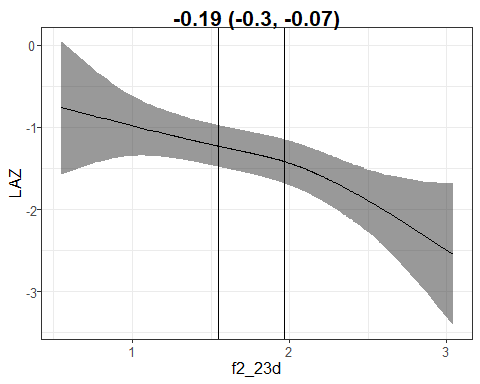
\includegraphics{stress-growth-lab-presentation_files/figure-beamer/unnamed-chunk-4-1.pdf}
\end{frame}

\begin{frame}{Exposure-response: Concurrent f2 23d and LAZ}
\protect\hypertarget{exposure-response-concurrent-f2-23d-and-laz}{}
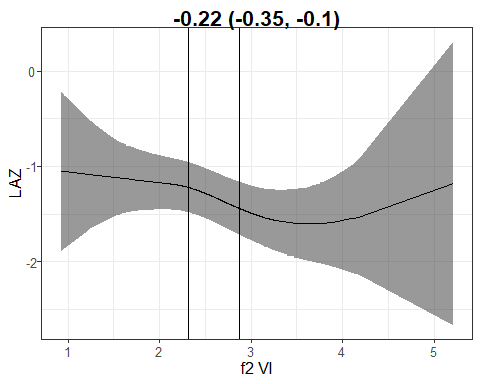
\includegraphics{stress-growth-lab-presentation_files/figure-beamer/unnamed-chunk-5-1.pdf}
\end{frame}

\begin{frame}{Exposure-response: Concurrent f2 VI and LAZ}
\protect\hypertarget{exposure-response-concurrent-f2-vi-and-laz}{}
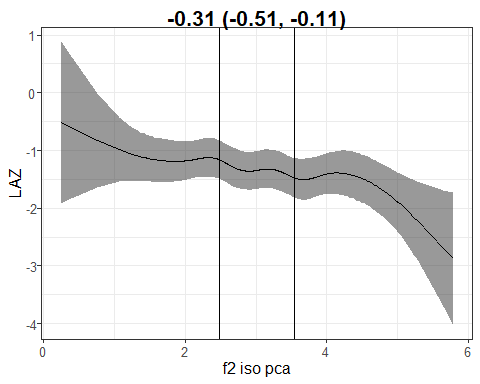
\includegraphics{stress-growth-lab-presentation_files/figure-beamer/unnamed-chunk-6-1.pdf}
\end{frame}

\begin{frame}{Exposure-response: Concurrent f2 iso pca and LAZ}
\protect\hypertarget{exposure-response-concurrent-f2-iso-pca-and-laz}{}
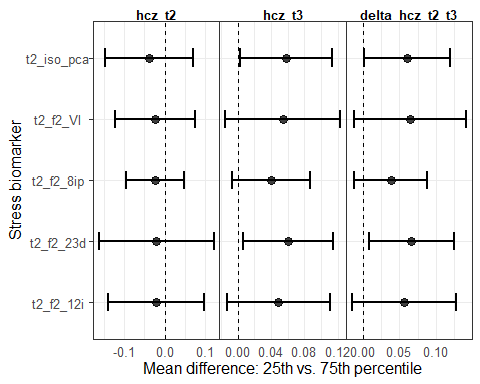
\includegraphics{stress-growth-lab-presentation_files/figure-beamer/unnamed-chunk-7-1.pdf}
\end{frame}

\begin{frame}{Primary findings - HCZ}
\protect\hypertarget{primary-findings---hcz}{}
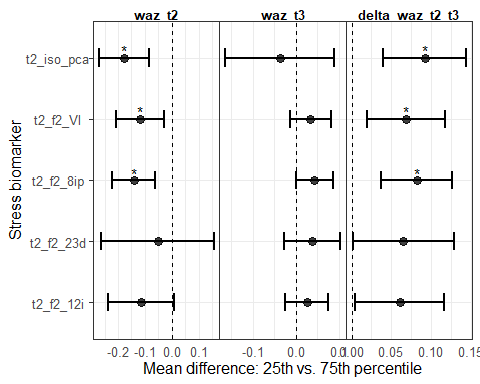
\includegraphics{stress-growth-lab-presentation_files/figure-beamer/unnamed-chunk-8-1.pdf}
\end{frame}

\begin{frame}{Primary findings - WAZ}
\protect\hypertarget{primary-findings---waz}{}
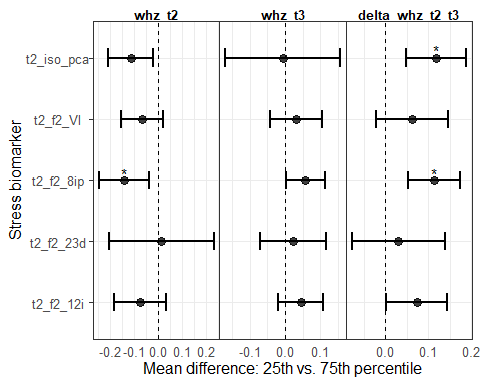
\includegraphics{stress-growth-lab-presentation_files/figure-beamer/unnamed-chunk-9-1.pdf}
\end{frame}

\begin{frame}{Primary findings - WHZ}
\protect\hypertarget{primary-findings---whz}{}
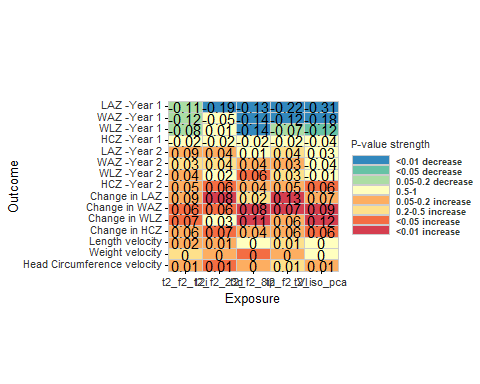
\includegraphics{stress-growth-lab-presentation_files/figure-beamer/unnamed-chunk-10-1.pdf}
\end{frame}

\begin{frame}{Primary findings: H2}
\protect\hypertarget{primary-findings-h2}{}
No associations significant after P-value correction with other growth
outcomes

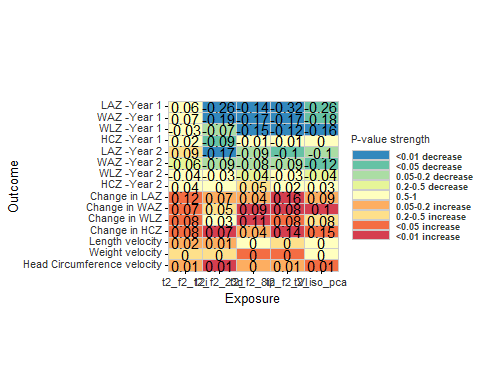
\includegraphics{stress-growth-lab-presentation_files/figure-beamer/unnamed-chunk-11-1.pdf}
\end{frame}

\begin{frame}{Primary findings: H3}
\protect\hypertarget{primary-findings-h3}{}
No associations significant after P-value correction with other growth
outcomes

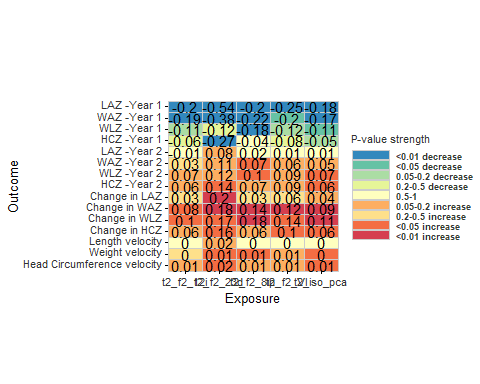
\includegraphics{stress-growth-lab-presentation_files/figure-beamer/unnamed-chunk-12-1.pdf}
\end{frame}

\begin{frame}{Primary findings: H4}
\protect\hypertarget{primary-findings-h4}{}
No associations significant after P-value correction with other growth
outcomes

\includegraphics{stress-growth-lab-presentation_files/figure-beamer/unnamed-chunk-13-1.pdf}
\end{frame}

\begin{frame}{Conclusions}
\protect\hypertarget{conclusions}{}
\begin{itemize}[<+->]
\tightlist
\item
  Consistent evidence of hypothesis that urinary F2-isoprostane measures
  are negatively associated with child growth.
\item
  F2-isoprostanes are a group of prostaglandin-like compounds that have
  been validated as a measure of oxidative stress, indicating oxidative
  stress is associated with decreased child growth.
\item
  Evidence that children with higher concentrations of urinary
  F2-isoprostane measures have faster growth velocity, evidence of
  catch-up growth or possible regression to the mean.
\item
  Possible alternative explanation? Children with low growth have higher
  F2-isoprostane measures (reverse causality), so we wouldn't expect an
  association between 14 month F2-isoprostane concentrations and 28
  month growth. Mild catch-up growth explains the positive association
  with growth trajectories.
\item
  Alternatively, some acute insult like diarrheal disease or failure to
  appropriately breastfeed leads to both reduced growth and increased
  oxidative stress. Chronic undernutrition or small stature, which would
  lead to maintained small stature at 28 months, has less of an impact
  on oxidative stress so there isn't an association 28 months growth.
  -Additional evidence for this: LAZ at 3 months not associated with
  F2-isoprostane measures
\item
  No strong evidence for other three hypotheses.
\end{itemize}
\end{frame}

\begin{frame}{Exploratory visualizations - Change in LAZ by quartile of
F2-23d}
\protect\hypertarget{exploratory-visualizations---change-in-laz-by-quartile-of-f2-23d}{}
\includegraphics{stress-growth-lab-presentation_files/figure-beamer/unnamed-chunk-14-1.pdf}
\end{frame}

\end{document}
